\begin{frame}{Nodal $hp$-version finite element methods}
  \begin{columns}
    \begin{column}{0.4\textwidth}
      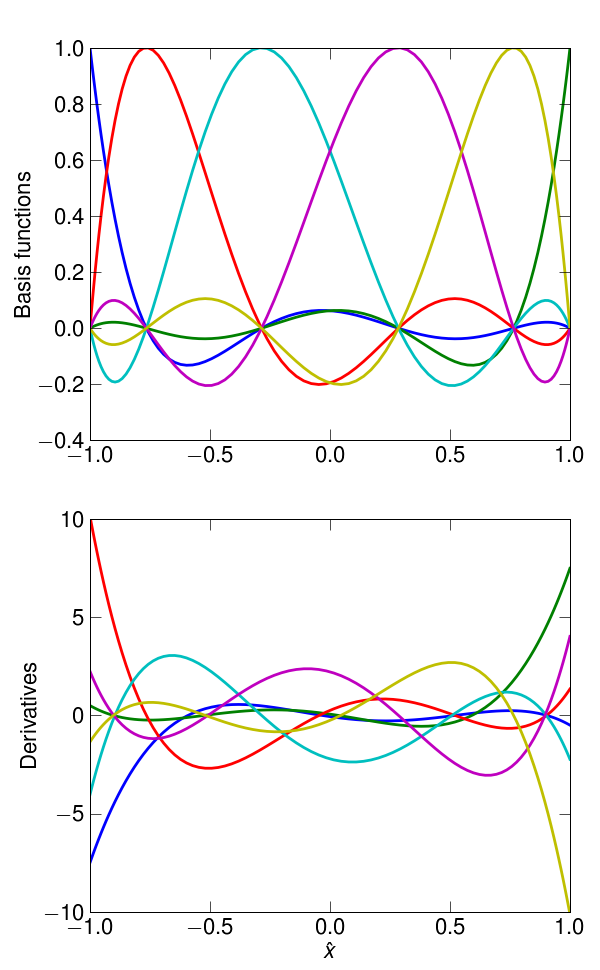
\includegraphics[width=\textwidth]{figures/lgl}
    \end{column}
    \begin{column}{0.6\textwidth}
      \begin{block}{1D reference element}
        \begin{itemize}
        \item Lagrange interpolants on Legendre-Gauss-Lobatto points
        \item Quadrature $\hat R$, weights $\hat W$
        \item Evaluation: $\hat B, \hat D$
        \end{itemize}
      \end{block}
      \vspace{-1em}
      \begin{block}{3D reference element}
      \vspace{-1em}
        \begin{align*}\label{eq:tprod}
          \begin{split}
            % \hat{\bm R} &= \hat R \otimes \hat R \otimes \hat R \\
            \hat{\bm W} &= \hat W \otimes \hat W \otimes \hat W \\
            \hat{\bm B} &= \alert<2>{\hat B \otimes \hat B \otimes \hat B} \\
          \end{split} &
          \begin{split}
            \hat{\bm D}_0 &= \alert<2>{\hat D \otimes \hat B \otimes \hat B} \\
            \hat{\bm D}_1 &= \alert<2>{\hat B \otimes \hat D \otimes \hat B} \\
            \hat{\bm D}_2 &= \alert<2>{\hat B \otimes \hat B \otimes \hat D} \\
          \end{split}
        \end{align*}
        \vspace{-1em}
        \begin{block}<2>{\alert{These tensor product operations \\ 
              are very efficient, 70\% of peak flop/s}}
        \end{block}
      \end{block}
    \end{column}
  \end{columns}
\end{frame}

\begin{frame}{Operations on physical elements}
  \begin{block}{Mapping to physical space}
    \vspace{-2em}
    \begin{gather*}
      x^e : \hat K \to K^e,\quad J^e_{ij} = \partial x_i^e/\partial \hat x_j, \quad (J^e)^{-1} = \partial \hat x/\partial x^e \\
    \end{gather*}
  \vspace{-2em}
  \end{block}
  \vspace{-2em}
  \begin{block}{Element operations in physical space}
  \vspace{-2em}
    \begin{align*}
      \bm B^e &= \hat{\bm B} \qquad \qquad \qquad \bm W^e = \hat{\bm W} \Lambda(\abs{J^e(\bm r)}) \\
      \bm D^e_i &= \Lambda\left(\frac{\partial \hat x_0}{\partial x_i}\right) \hat{\bm D}_0
      + \Lambda\left(\frac{\partial \hat x_1}{\partial x_i}\right) \hat{\bm D}_1
      + \Lambda\left(\frac{\partial \hat x_2}{\partial x_i}\right) \hat{\bm D}_2 \\
      (\bm D^e_i)^T &= \hat{\bm D}_0^T \Lambda\left(\frac{\partial \hat x_0}{\partial x_i}\right)
      + \hat{\bm D}_1^T \Lambda\left(\frac{\partial \hat x_1}{\partial x_i}\right)
      + \hat{\bm D}_2^T \Lambda\left(\frac{\partial \hat x_2}{\partial x_i}\right)
    \end{align*}
  \end{block}
  \vspace{-2em}
  \begin{block}{Global problem is defined by assembly}
  \vspace{-2em}
  \begin{equation*}
    F(u) =
    \sum_e \EE_e^T \Big[ (\bm B^e)^T \bm W^e \Lambda({\color{green!70!black} f_0(u^e,\nabla u^e)})
    + \sum_{i=0}^d(\bm D_i^e)^T \bm W^e \Lambda({\color{green!70!black} f_{1,i}(u^e,\nabla u^e)}) \Big] = \bm 0
  \end{equation*}
  where $u^e = \bm B^e \EE^e u$ and $\nabla u^e = \{\bm D_i^e \EE^e u\}_{i=0}^2$
  \end{block}
\end{frame}
